\documentclass[a4paper,11pt]{article}
\usepackage[T1]{fontenc}
\usepackage[english]{babel}
\usepackage{amsmath}
\usepackage{amsfonts}
\usepackage{color}
\usepackage{graphicx}
\usepackage{subfigure}
\usepackage{epsf}
\usepackage[left=2cm,right=2cm,top=2cm,bottom=2cm]{geometry}
\usepackage{float}
\usepackage{lmodern} 
\usepackage[table]{xcolor}
\usepackage{multirow}
\usepackage{listings} 
\usepackage[justification=centering]{caption}
\usepackage{hyperref}

%ttfamily

\lstset{% 
language=r, 
basicstyle=\scriptsize, 
keywordstyle=\color{blue}\bfseries, 
commentstyle=\color{black!20!green}, 
stringstyle=\color{red}, 
numbers=left,
numberstyle=\tiny,
frame=\lines
} 

\title{%
    \begin{minipage}\linewidth
        \centering
        \Huge{\textbf{Application of machine learning methods for claim prediction in car insurance data}}
        \vskip75pt
        \huge{Report for Workshop I - "Actuarial science" \\ Master of Data Science, University of Luxembourg}
    \end{minipage}
}

%\title{\Huge{\textbf{Simulation de variables aléatoires Implémentations en Matlab}}}
\author{\Large{Barbara {\sc Gendron-Audebert}}}
\date\today

\begin{document}
\rowcolors{2}{gray!20}{white}
\maketitle
\newpage

% --------------------------------------------------------------

% Attention  IL FAUT VULGARISER DAVANTAGE !!!! 

\section{Data and related insurance problem} 

\subsection{Dataset description}

This dataset contains exactly 10000 samples, and 19 columns.\\

\noindent The credit score reflect the ability for a policyholder to pay for his debts. The higher the score, the more creditworthy the policyholder is. In car insurance, it is has been observed that this parameter has a significant influence on the insurance rate.\\
{\tt DUIS} refers to DUI, which stands for \textsl{driving under the influence} (whether it be alcohol or drugs).

% Trier par ordre alphabetique du type
\begin{table}[ht]
    \begin{tabular}[t]{|lcc|}
        \rowcolor{orange!30}
\hline
\textbf{Variable}           & \textbf{Type}      & \textbf{Value ranges (if meaningful)}     \\
\hline
VEHICLE OWNERSHIP   & Binary    & 0 or 1                     \\
MARRIED             & Binary    & 0 or 1                     \\
CHILDREN            & Binary    & 0 or 1                    \\
OUTCOME             & Binary    & 0 or 1                     \\
AGE                 & Category    & 16-25, 26-39, 40-64, 65+      \\
GENDER              & Category    & female, male                  \\
RACE                & Category    & majority, minority            \\
DRIVING EXPERIENCE  & Category    & 0-9y, 10-19y, 20-29y, 30y+     \\
EDUCATION           & Category    & high school, none, university \\
INCOME              & Category    & middle class, poverty, upper class, working class \\
VEHICLE TYPE        & Category    & sedan, sports car             \\
VEHICLE YEAR        & Category    & after 2015, before 2015       \\
CREDIT SCORE        & Float     & From 0.0534 to 0.9608       \\
ID                  & Integer   & --                \\
POSTAL CODE         & Integer   & --             \\ 
ANNUAL MILEAGE      & Integer   & From 2000 to 22000               \\ 

SPEEDING VIOLATIONS & Integer   & From 0 to 22                   \\
DUIS                & Integer   & From 0 to 6                      \\ 
PAST ACCIDENTS      & Integer   & From 0 to 15                    \\  

\hline
    \end{tabular}
\centering
\caption{A short description of the covariates, along with some insights about categorical variables.}
\end{table}%

\subsection{The insurance context}

\section{Preliminary analysis of the data}
\subsection{Exploratory data analysis}

In this part I will conduce an exploratory data analysis focusing on the following points:
\begin{itemize}
    \item distribution of variables for numerical ones
    \item distribution of numerical features depending on the {\tt OUTCOME} value
    \item classes distributions depending on the {\tt OUTCOME} value for categorical features
\end{itemize}

\subsubsection{Distribution of variables and classes balance}

\begin{figure}[!h]
    \centering
    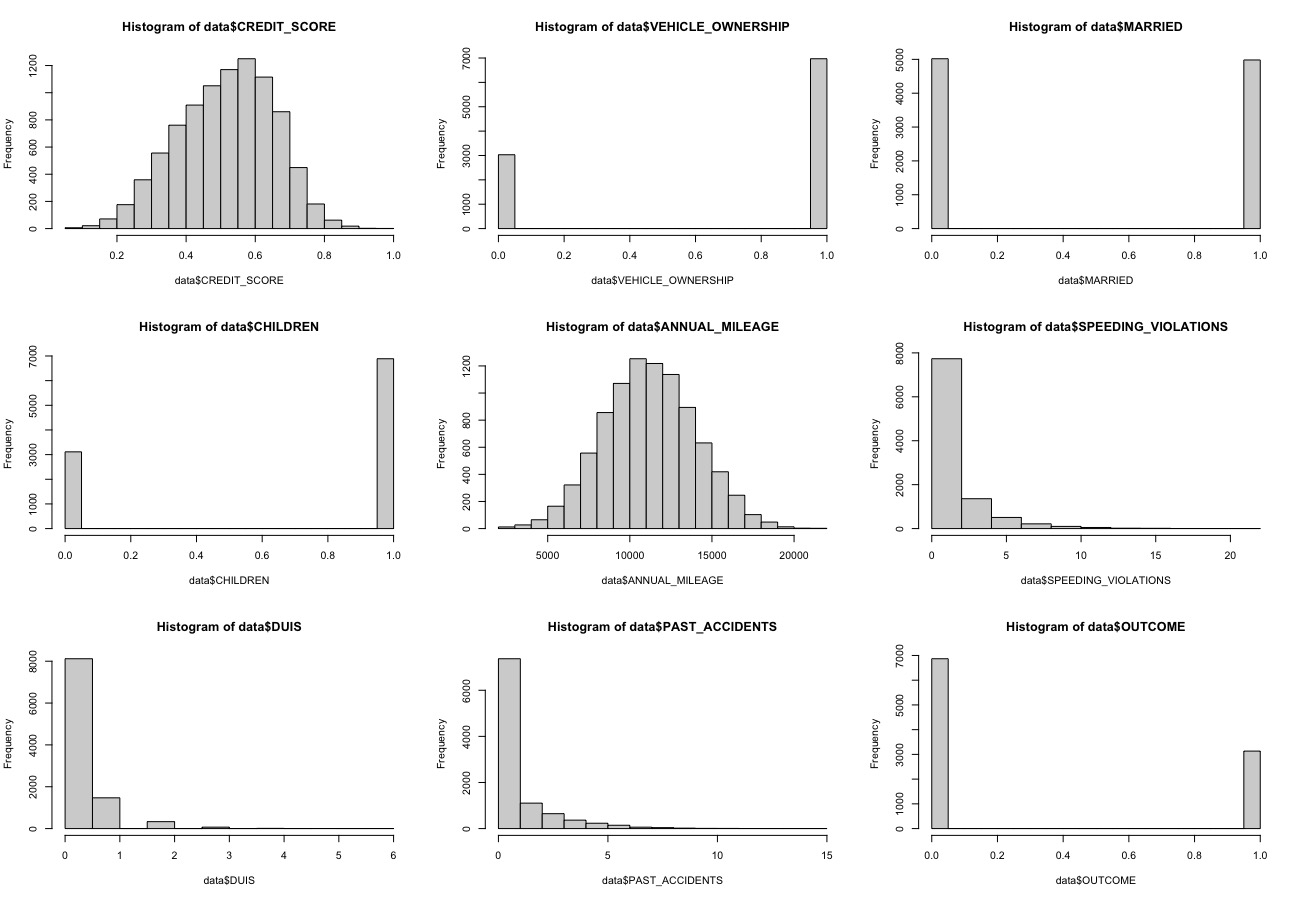
\includegraphics[scale=0.35]{eda.jpeg}
    \caption{Histograms of the numerical variables.}
\end{figure}

\subsubsection{Distribution of numerical features depending on the {\tt OUTCOME} value}

The following figure aims at showing how different is the distribution of a certain numerical feature with respect to the {\tt OUTCOME} value. For this purpose, I used violin plots, which are basically boxplots enhanced by showing the shape of the distribution.

\subsubsection{Classes distributions depending on the {\tt OUTCOME} value for categorical features}

\begin{figure}[!h]
    \centering
    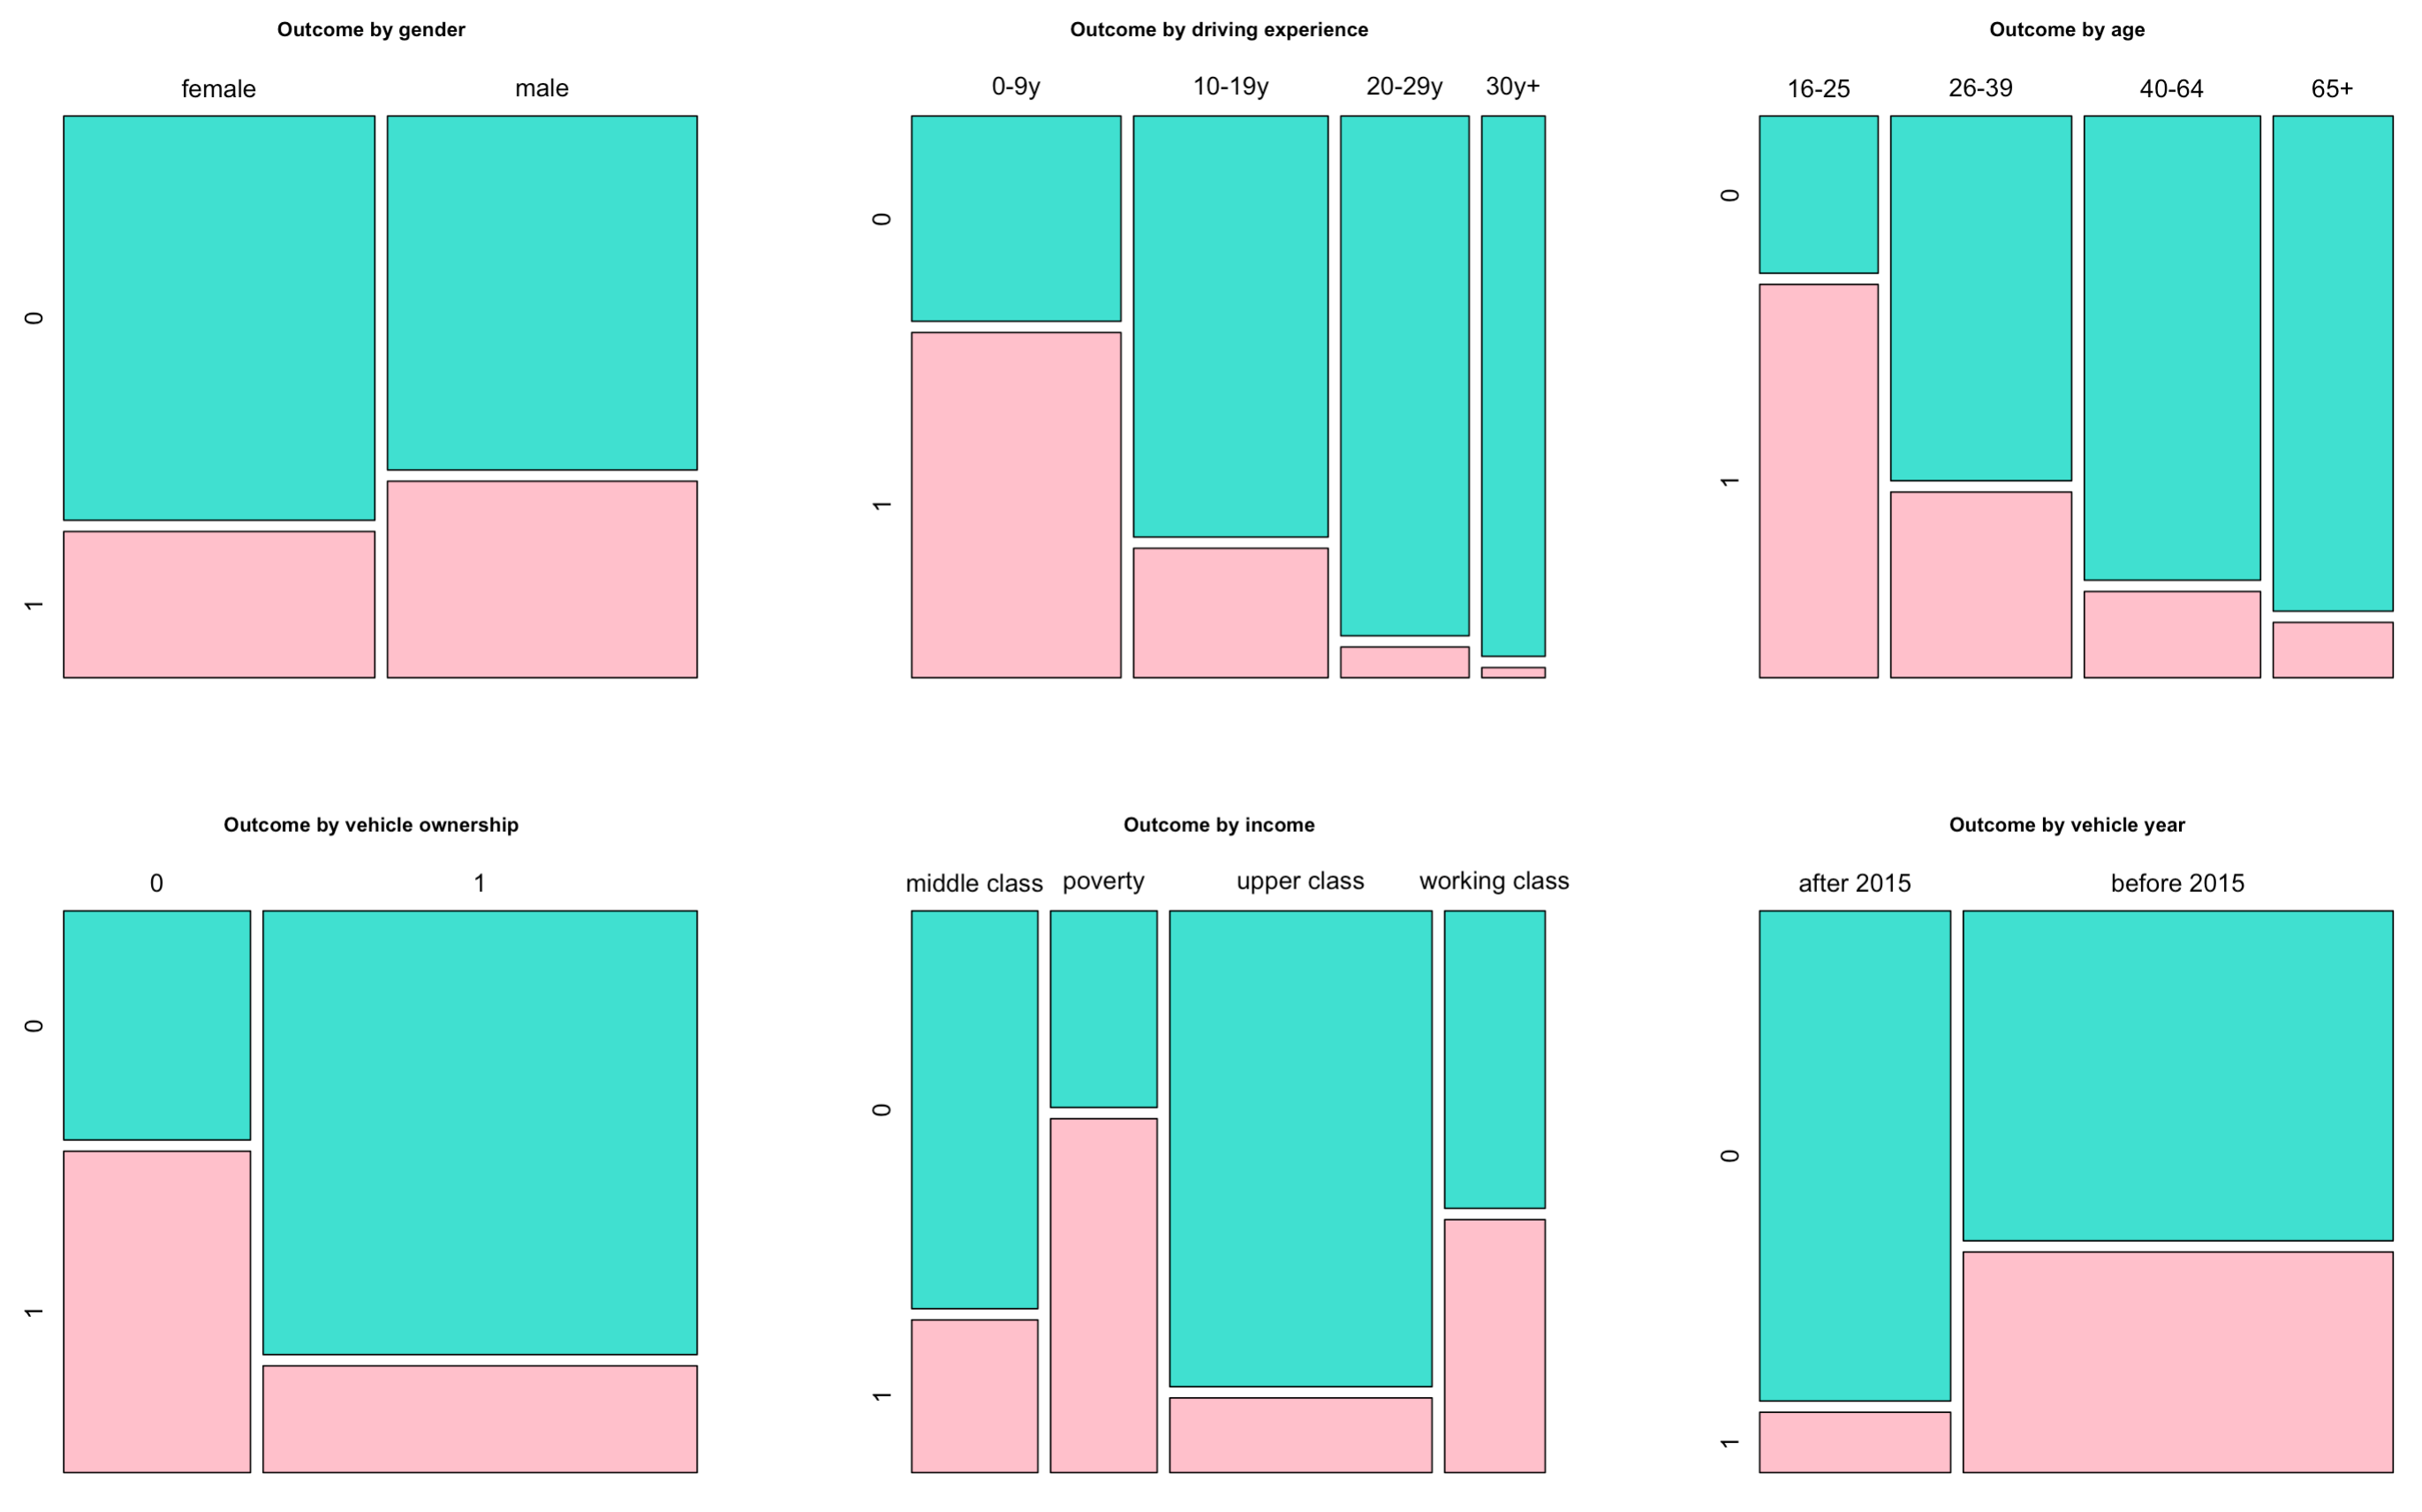
\includegraphics[scale=0.3]{eda-report.png}
    \caption{Value counts of categorical features with respect to the {\tt OUTCOME} value.}
\end{figure}

\subsubsection{Dataset summary and completeness of the dataset}

Using the {\tt summary()} R function, we observe that the variables {\tt CREDIT SCORE} and {\tt ANNUAL MILEAGE} respectively have 982 and 957 NA's values. This represents approximately 1\% of the whole data for each variable, that's why we can consider simply delete them. Thus, the remaining dataset contains 8149 rows. 

\section{Brief description of the models used}


\section{Analysis of the results and conclusion}
\rowcolors{2}{white}{white}
\begin{table}[ht]
    \begin{tabular}[t]{|c|ccccc|}
\hline
\textbf{Model} & \textbf{Accuracy} & \textbf{Sensitivity} & \textbf{Specificity} & \textbf{PPV} & \textbf{NPV} \\
\hline
Logistic regression         & \underline{0.8245} & 0.8629 & \underline{0.7334} & \underline{0.8850} & 0.6923 \\
Decision Tree Classifier    & 0.8164          & 0.8534 & 0.7252 & 0.8844 & 0.6675 \\
Random Forest Classifier    & \underline{0.8245} & \underline{0.8719} & 0.7206 & 0.8725 & 0.7197 \\
XGBoost                     & 0.8164          & 0.8844 & 0.6675 & 0.8534 & \underline{0.7252} \\
\hline
    \end{tabular}
\centering
\caption{A sum-up table of the classification metrics for each model. PPV stands for Predicted Positive Values and NPV stands for Negative Predicted Values.}
\end{table}%

\end{document}